\documentclass[a4paper,12pt]{report}

\usepackage{float}
\usepackage{hyperref}
\usepackage{amsmath}
\usepackage{listings}
\usepackage{graphicx}

\begin{document}
\tableofcontents

\title{relazione}

\chapter{Analisi dei requisiti}
\section{Intervista}
Vogliamo sviluppare un social network puramente testuale.
Gli \textbf{utenti} possono iscriversi e disicriversi. Al momento dell'iscrizione l'utente inserisce un username identificativo e opzionalmente le sue generalità(nome, cognome, data di nascita, proprio domicilio). Inoltre decide una password che utilzzerà per autenticarsi al social network.
L'utente può cambiare la sua password ma non può riutilizzare una password precedente.
Ogni utente può pubblicare dei \textbf{post}. Un post consiste in un titlo, un testo scritto, opzionalmente accompagnato da una locazione decisa dall'autore (cioè l'utente che ha scritto il post). I post possono essere commentati dagli utenti.
Ogni utente può mettere \textbf{like} e dislike a post e commenti. Ricevendo reazioni ai propri post e commenti gli utenti si costruiscono una reputazione, ciè un indice frutto della somma algebrica tra like e dislike.
Gli utenti inoltre possono \textbf{seguire} altri utenti e smettere di seguirli. Sarà possibile avere uno storico di queste operazioni. 
Il social fornirà ad ogni utente un feed, cioè una sequeza di post pubblicati dagli utenti da lui seguiti.
Gli utenti possono chattare con altri utenti. Le \textbf{chat} si compongono di messaggi inviati dai membri di quella chat. Ogni \textbf{messaggio} ha un suo autore, un timestamp di invio, un testo ed può citare un post o commento. Ogni messaggio inoltre può essere in risposta ad un altro messaggio di quella chat. 
Ogni utente può creare una \textbf{chat}. Ogni chat ha uno o più membri amministratori. Gli \textbf{amministratori} possono far entrare nuovi membri nelle chat di cui sono amministratori. Gli amministratori hanno diritto di cacciare degli utenti dalla chat, eventualmente comunicando una motivazione. Gli utenti possono uscire volontariamente dalle chat a cui appartengono. Gli utenti che escono volontariamente dalla chat possono lasciare una motivazione del loro gesto. 
\section{Definizioni}
\begin{itemize}
    \item Utente: un iscritto al nostro social network.  
    \item Post: un testo scritto da un utente 
    \item Autore di un post: l'utente che ha scritto il post
    \item Commento: un post che fa riferimento ad un altro post (detto post padre)
    \item Like: è una segnalazione di gradimento ad un post
    \item Dislike: l'opposto di un like
    \item Reputazione di un utente: la differenza tra like e dislike complessivi dei post scritti dall'utente
    \item Messaggio: un testo scritto da un utente con destinatario una chat 
    \item Chat: una sequenza di messaggi
    \item Membro di una chat: un utente che fa parte della chat  
    \item Regione: un luogo geografico
    \item Amministratore di una chat: un utente che può aggiungere e rimuovere utenti dalla chat
    \item Creatore di una chat: l'utente che ha creato la chat, in altre parole il primo membro di una chat (nonchè il primo amministratore)
\end{itemize}


\subsection{Operazioni utente}
\begin{itemize}
    \item Creare un nuovo utente
    \item Cambiare password utente
    \item Seguire utente
    \item Mandare un messaggio
    \item Postare e commentare
    \item Like/dislike
    \item Creare un gruppo
    \item Aggiungere utente al gruppo
    \item Vedere tutti i post in ordine cronologico (feed)
    \item Vedere utenti che hanno messo like a un post
    \item Leggere messaggi di una chat
    \item Login utente
    \item Aggiungere location a tabella location
    \item Vedere profilo utente (location, reputazione, post \ldots)
    \item Dare diritti amministratore ad un utente in un gruppo
\end{itemize}

\chapter{Progettazione Concettuale}
\section{Utenti}
L'entità utente ha come unico identificatore lo username. Per permettere agli utenti di seguire altri utenti abbiamo creato una associazione ad anello SEGUIRE. Però per permettere la creazione di uno storico dei seguiti abbiamo reificato questa associazione.
\subsection{Login e logout}
Ogni qual volta l'utente entra nel social network viene creata una istanza di STORICO\_ACCESSO. Non riusciamo ad esprimere il vincolo secondo cui il timestamp di logout deve essere successivo a quello quello di login. 
Vogliamo invece permettere accessi in intervalli sovrapposti da parte di uno stesso utente. 

\section{Chat e membri della chat}
Quando un utente entra a fare parte di una chat viene creata una istanza di MEMBRO, identificata dalla tripla (utente, chat, data di entrata). Rimane inespresso il vincolo secondo cui un utente non far parte contemporaneamente della stessa chat. Quando un membro esce dalla chat la sua istanza non viene eliminata ma semplicemente viene creata una istanza di USCITA, la quale verrà referenziata dal membro uscito.
Modelliamo i membri amministratori come sottotipi di membri. Ogni membro ha un membro amministratore che lo ha aggiunto alla chat tranne il creatore della chat. Non riusciamo ad esprimere tramite E/R il vincolo secondo cui gli amministratori possono aggiungere utenti alle chat di cui amministratori.
\subsection{Uscita dalla chat}
L'uscita volontaria dalla chat è rapresentata dal sottotipo di USCITA chiamato VOLONTARIA. Quando invece un amministratore caccia un membro allora si crea una istanza di tipo ESILIO, la quale referenzia l'amministratore responsabile della cacciata.

\section{Regione}
Una regione può far parte di una ed una sola regione più grande, mentre una regione può contenere delle regioni più piccole. Esprimiamo questi vincoli con una relazione ad anello. Si viene perciò a formare un albero (o una foresta di alberi) che esprimono le gerarchie delle regioni geografiche. Lasciamo però inespresso il vincolo secondo cui non si debbano formare dei cicli all'interno di questa foresta, vincolo che abbiamo intenzione di imporre a livello applicativo. 

\section{Password}
Ogni utente ha uno storico di password che ci permette di impedire all'utente di riutilizzare password passate. Questo vincolo è espresso imponendo come identificatore della entità \texttt{STORICO\_PASSWORD} la tupla \texttt{(Password, UTENTE)}. Imponiamo inoltre il vincolo secondo cui un utente non può avere contemporaneamente due password creando l'identificatore \texttt{(Password, DataInserimento)}.

\section{Contenuto (post e commenti)}
Abbiamo modellizzato post e commenti in una gerarchia totale ed esclusiva dove i post veri e propri (cioè quelli pubblicati \textbf{non} in risposta a qualche altro contenuto) sono istanze della sottoclasse \texttt{POST}, mentre i commenti (cioè quei contenuti in risposta ad altri contenuti) sono rappresentati dall'entità figlia \texttt{COMMENTO}. Questa entità è legata a \texttt{CONTENUTO} dalla relazione \texttt{RISPOSTA}, che indica a quale contenuto il commento fa rifermento.
Per modellizzare la possibilità da parte degli utenti di mettere like e dislike ai contenuti abbiamo creato la relazione \texttt{REAZIONE} il cui attributo \texttt{LikeDislike} indica se la reazione è un like o un dislike. L'attributo \texttt{Timestamp} indica il momento temporale in cui l'utente ha espresso la sua reazione riguardo al contenuto. 

\section{Schema concettuale finale}
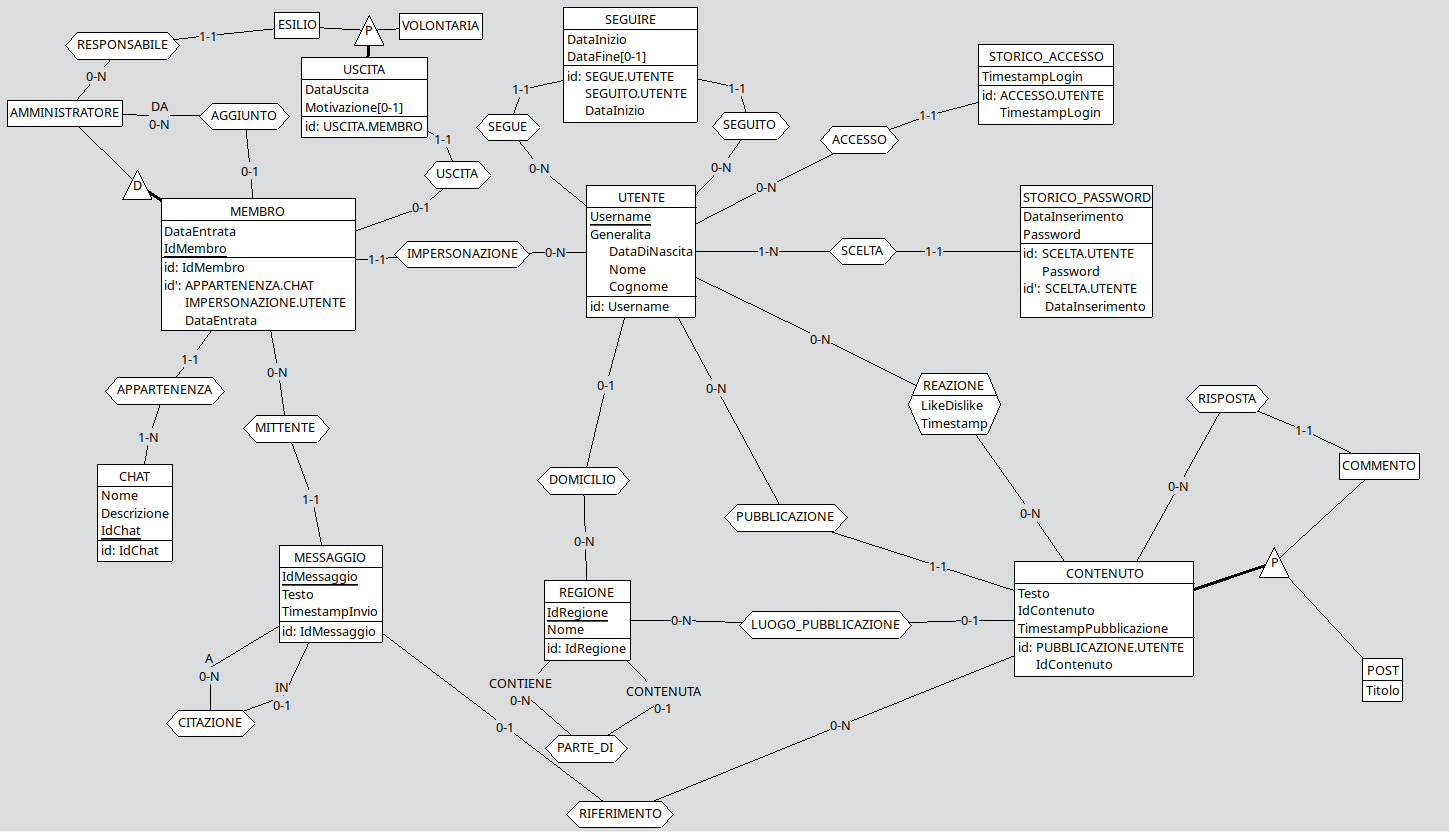
\includegraphics[scale=0.6, angle=90]{./img/concettuale.png}
\chapter{Progettazione logica}
\section{Stima del volume dei dati}

\begin{itemize}
  \item UTENTE, E, 1000
  \item SCELTA, R, 5000
  \item STORICO\_PASSWORD, E, 5000
  \item SEGUIRE, R, 100.000
  \item SEGUE, E, 100.000
  \item SEGUIRE E, 100.000
  \item MEMBRO, E, 20000
  \item AMMINISTRATORE, E, 4000
  \item PUBBLICAZIONE, R, 20000
  \item POST, E, 20000
  \item COMMENTO, E, 200.000
  \item REAZIONE, R, 2.000.000
  \item IMPERSONAZIONE, R, 20000
  \item APPARTENENZA, R, 20000
  \item CHAT, E, 2000 
  \item AGGIUNTO, R, 20000 
  \item MESSAGGIO, E, 300000
  \item MITTENTE, R, 300000
  \item CITAZIONE, R, 10000
  \item DOMICILIO, R, 100
  \item REGIONE, E, 150.000.000
  \item PARTE\_DI, R, 150.000.000

\end{itemize}

\section{Tabelle degli accessi}

\subsection{Creare un nuovo utente} \label{nuovo_utente}
\paragraph{Descrizione} Aggiungere alla tabella degli utenti una nuova riga e assegnargli una password 
\paragraph{Frequenza} 10 / g 
\begin{table}[H]
\paragraph{Tavola degli accessi\newline}
\begin{tabular}{|c|c|c|c|}
\hline
Concetto          & Costrutto & Accessi & Tipo \\ \hline
UTENTE            & E         & 1       & W    \\ \hline
SCELTA           & A         & 1       & W    \\ \hline
STORICO\_PASSWORD & E         & 1       & W    \\ \hline
\textit{Gerarchia regioni \ref{aggiungere_regione}} &  & 14      &      \\ \hline 
\textit{TOTALE}   &           & 20       &      \\ \hline
\end{tabular}
\end{table}
\subsection{Cambiare password} \label{cambio_password}
\paragraph{Descrizione} Aggiungere alla tabella dello storico password una nuova riga. 
\paragraph{Frequenza} 1 / 60 g 
\begin{table}[H]
\paragraph{Tavola degli accessi\newline}
\begin{tabular}{|c|c|c|c|}
\hline
Concetto          & Costrutto & Accessi & Tipo \\ \hline
UTENTE            & E         & 1       & R    \\ \hline
SCELTA            & A         & 1       & W    \\ \hline
STORICO\_PASSWORD & E         & 1       & W    \\ \hline
\textit{TOTALE}   &           & 5       &      \\ \hline
\end{tabular}
\end{table}
\subsection{Autenticazione dell'utente all'interno del social network tramite username e password} \label{autenticazione}
\paragraph{Descrizione} Si controlla se esiste istanza di STORICO\_PASSWORD contentente l'username e la password inserite
\paragraph{Frequenza} 10 / g
\begin{table}[H]
\paragraph{Tavola degli accessi\newline}
\begin{tabular}{|c|c|c|c|}
\hline
Concetto          & Costrutto & Accessi & Tipo \\ \hline
UTENTE            & E         & 1       & R    \\ \hline
SCELTA            & A         & 1       & R    \\ \hline
STORICO\_PASSWORD & E         & 5       & R    \\ \hline
ACCESSO           & A         & 1       & W    \\ \hline
STORICO\_ACCESSO  & E         & 1       & W    \\ \hline
TOTALE            &           & 11      &      \\ \hline
\end{tabular}
\end{table}
\subsection{Seguire un utente} \label{follow}
\paragraph{Descrizione} Si aggiunge una istanza alla tabella SEGUIRE avente come chiave la tupla (utente seguace, utente seguito)
\paragraph{Frequenza} 2 / g
\paragraph{Tavola degli accessi}
Trattata nell'analisi delle ridondanze.
\paragraph{Schema di navigazione\newline}
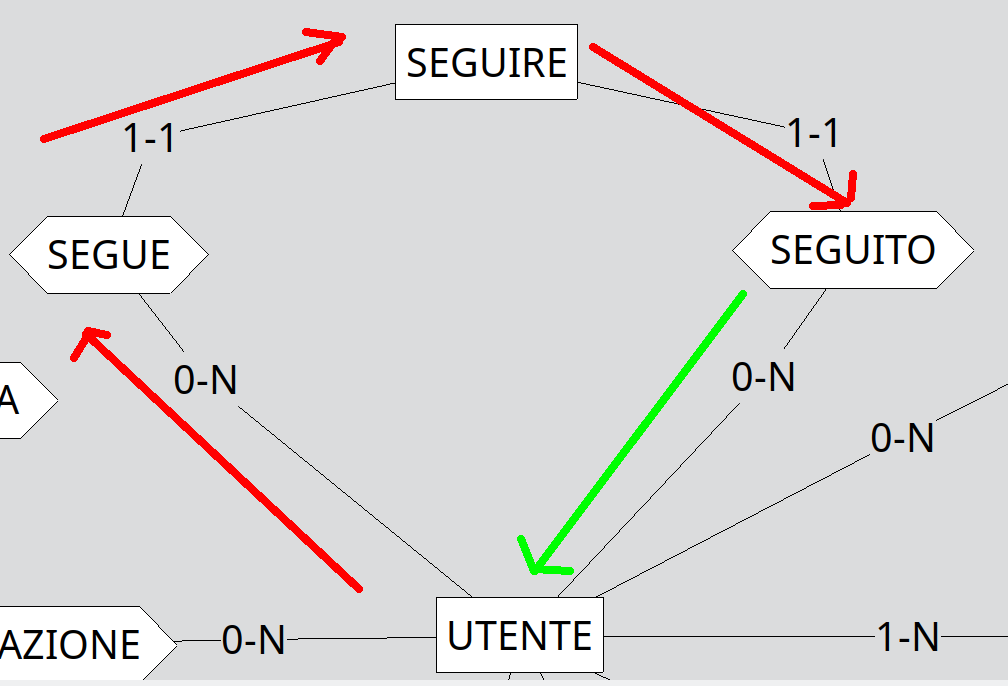
\includegraphics[scale=0.5]{./img/seguire.png}
\subsection{Smettere di seguire un utente} \label{unfollow}
\paragraph{Descrizione} Si accede all'istanza di SEGUIRE identificata dalla tupla (utente seguace, utente seguito) e si aggiunge assegna al campo DataFine la data attuale.
\paragraph{Tavola degli accessi}
Trattata nell'analisi delle ridondanze.

\paragraph{Frequenza} 1 / 10 g
\begin{table}[H]
\paragraph{Tavola degli accessi\newline}
\begin{tabular}{|c|c|c|c|}
\hline
Concetto & Costrutto & Accessi & Tipo \\ \hline
UTENTE   & E         & 1       & R    \\ \hline
SEGUE    & A         & 1       & R    \\ \hline
SEGUIRE  & E         & 1       & W    \\ \hline
UTENTE   & E         & 1       & R    \\ \hline
TOTALE   &           & 5       &      \\ \hline
\end{tabular}
\end{table}
\subsection{Creare una nuova chat} \label{nuova_chat}
\paragraph{Descrizione} Viene creato una nuova istanza di CHAT e un primo membro amminstratore della chat.
\paragraph{Frequenza} 1 / 20 g
\begin{table}[H]
\paragraph{Tavola degli accessi\newline}
\begin{tabular}{|c|c|c|c|}
\hline
Concetto       & Costrutto & Accessi & Tipo \\ \hline
UTENTE         & E         & 1       & R    \\ \hline
IMPERSONAZIONE & A         & 1       & W    \\ \hline
AMMINISTRATORE & E         & 1       & W    \\ \hline
APPARTENENZA   & A         & 1       & W    \\ \hline
CHAT           & E         & 1       & W    \\ \hline
TOTALE         &           & 9       &      \\ \hline
\end{tabular}
\end{table}
\paragraph{Schema di navigazione\newline}
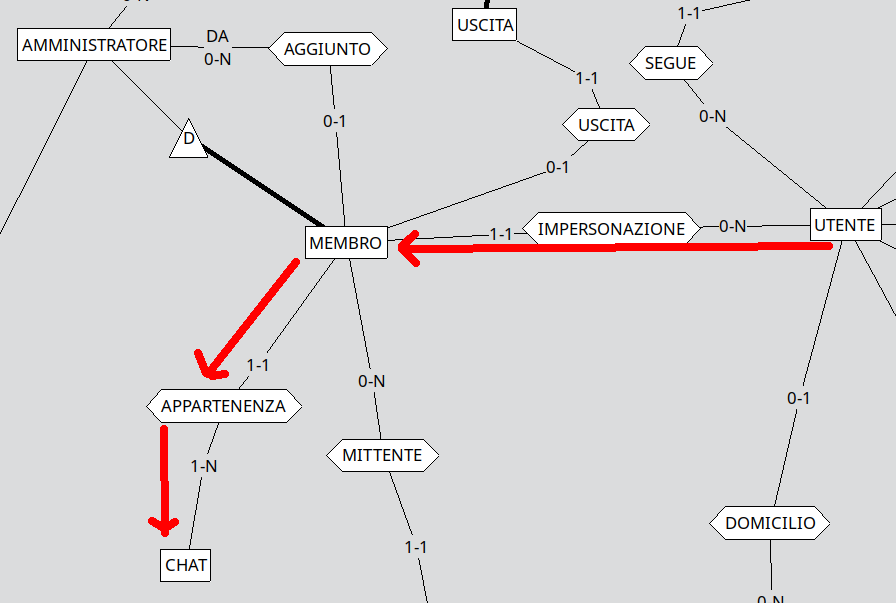
\includegraphics[scale=0.5]{./img/creare_chat.png}
\subsection{Postare e commentare} \label{postare}
\paragraph{Descrizione}
Aggiunge una nuova riga alla tabella CONTENUTO.
\paragraph{Frequenza} 10 / g
\begin{table}[H]
\paragraph{Tavola degli accessi\newline}
\begin{tabular}{|c|c|c|c|}
\hline
Concetto             & Costrutto & Accessi & Tipo \\ \hline
CONTENUTO            & E         & 1       & W    \\ \hline
PUBBLICAZIONE        & A         & 1       & W    \\ \hline
UTENTE               & E         & 1       & R    \\ \hline
LUOGO\_PUBBLICAZIONE & A         & 1       & W    \\ \hline
REGIONE              & E         & 1       & R    \\ \hline
RISPOSTA             & A         & 1       & W    \\ \hline
CONTENUTO            & E         & 1       & R    \\ \hline
TOTALE               &           & 11      &      \\ \hline
\end{tabular}
\end{table}
\subsection{Reagire con like/dislike a post e commenti} \label{like}
\paragraph{Descrizione} Si aggiunge una istanza alla tabella reazione con identificatore la tupla (utente, contenuto) e nel campo LikeDislike +1 se è un like, -1 se è un dislike.
\paragraph{Frequenza} 80 / g
\paragraph{Tavola degli accessi}  
Trattata nell'analisi delle ridondanze.
\subsection{Leggere un post} \label{leggere_post}
\paragraph{Descrizione} Si mostrano il contentuto, l'ora di pubblicazione, l'autore, i commenti, il numero di like netto (cioè la somma algebrica dei like e dislike), se presente il luogo di pubblicazione.
\paragraph{Frequenza} 100 / g
\paragraph{Tavola degli accessi}  
Trattata nell'analisi delle ridondanze.
\subsection{Scorrere il post pubblicati dagli utenti seguiti (feed)} \label{feed}
\paragraph{Descrizione} Questa operazione mostra in ordine cronologico i titoli, il numero di like netto e l'autore dei post pubblicati dagli utenti seguiti.
\paragraph{Frequenza} 40 / g
\paragraph{Tavola degli accessi}  
Trattata nell'analisi delle ridondanze.
\paragraph{Schema di navigazione\newline}
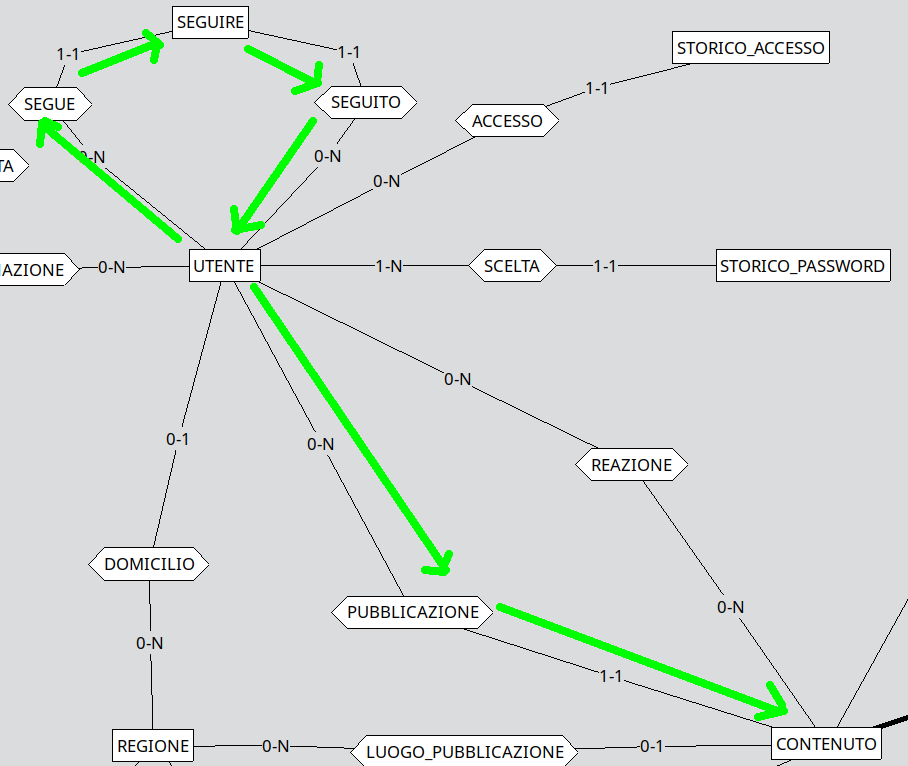
\includegraphics[scale=0.5]{./img/feed.png}
\subsection{Vedere il profilo di un utente} \label{vedere_profilo}
\paragraph{Descrizione} Si mostrano nome, cognome, data di nascita, location e la sua reputazione.
\paragraph{Frequenza} 5 / g
\paragraph{Tavola degli accessi}  
Trattata nell'analisi delle ridondanze.
\subsection{Vedere i contenuti pubblicati da un utente} \label{vedere_post_utente}
\paragraph{Descrizione} Si mostrano tutti i contenuti che hanno come autore l'utente considerato
\paragraph{Frequanza} 1 / g
\begin{table}[H]
\paragraph{Tavola degli accessi\newline}
\begin{tabular}{|c|c|c|c|}
\hline
Concetto      & Costrutto & Accessi & Tipo \\ \hline
UTENTE        & E         & 1       & R    \\ \hline
PUBBLICAZIONE & A         & 20      & R    \\ \hline
CONTENUTO     & E         & 20      & R    \\ \hline
TOTALE        &           & 41      &      \\ \hline
\end{tabular}
\end{table}
\subsection{Scrivere un messaggio nella chat} \label{scrivere_messaggio}
\paragraph{Descrizione} Si aggiunge una istanza nella tabella MESSAGGIO con una referenza esterna al membro autore.
\paragraph{Frequenza} 50 / g 
\begin{table}[H]
\paragraph{Tavola degli accessi\newline}
\begin{tabular}{|c|c|c|c|c|}
\hline
Concetto    & Costrutto & Accessi & Tipo \\ \hline
MEMBRO      & E         & 1       & R    \\ \hline
MITTENTE    & A         & 1       & W    \\ \hline
MESSAGGIO   & E         & 1       & W    \\ \hline
CITAZIONE   & A         & 1       & W    \\ \hline
MESSAGGIO   & E         & 1       & R    \\ \hline
RIFERIMENTO & A         & 1       & W    \\ \hline
CONTENUTO   & E         & 1       & R    \\ \hline
TOTALE      &           & 11      &      \\ \hline
\end{tabular}
\end{table}
\subsection{Uscire volontariamente dalla chat} \label{uscire_volontariamente}
\paragraph{Descrizione} Nell'istanza del membro che sta uscendo si aggiunge una referenza ad una nuova istanza USCITA di tipo VOLONTARIA.
\paragraph{Frequenza} 1 / 100 g 
\begin{table}[H]
\paragraph{Tavola degli accessi\newline}
\begin{tabular}{|c|c|c|c|}
\hline
Concetto   & Costrutto & Accessi & Tipo \\ \hline
MEMBRO     & E         & 1       & W    \\ \hline
USCITA     & A         & 1       & W    \\ \hline
VOLONTARIA & E         & 1       & W    \\ \hline
TOTALE     &           & 6       &      \\ \hline
\end{tabular}
\end{table}
\subsection{Elencare i membri attuali della chat} \label{membri_chat}
\paragraph{Descrizione} Vengono elencati gli username, ruolo e data di entrata degli utenti membri della chat.
\paragraph{Frequenza} 1 / g
\begin{table}[H]
\paragraph{Tavola degli accessi\newline}
\begin{tabular}{|c|c|c|c|}
\hline
Concetto     & Costrutto & Accessi & Tipo \\ \hline
CHAT         & E         & 1       & R    \\ \hline
APPARTENENZA & A         & 20      & R    \\ \hline
MEMBRO       & E         & 20      & R    \\ \hline
TOTALE       &           & 41      &      \\ \hline
\end{tabular}
\end{table}
\subsection{Leggere i messaggi della chat} \label{leggere_messaggi}
\paragraph{Descrizione} Ordinati dal più recente al più vecchio vengono mostrati il contenuto dei messaggi, il mittente, un eventuale messaggio citato e un eventuale contenuto in riferimento. Verranno ignorati i messaggi eliminati.
\paragraph{Frequenza} 90 / g
\begin{table}[H]
\paragraph{Tavola degli accessi\newline}
\begin{tabular}{|c|c|c|c|}
\hline
Concetto     & Costrutto & Accessi & Tipo \\ \hline
CHAT         & E         & 1       & R    \\ \hline
APPARTENENZA & A         & 20      & R    \\ \hline
MEMBRO       & E         & 20      & R    \\ \hline
MITTENTE     & A         & 300     & R    \\ \hline
MESSAGGIO    & E         & 300     & R    \\ \hline
CITAZIONE    & A         & 300     & R    \\ \hline
MESSAGGIO    & E         & 300     & R    \\ \hline
RIFERIMENTO  & A         & 300     & R    \\ \hline
CONTENUTO    & E         & 300     & R    \\ \hline
TOTALE       &           & 1841    &      \\ \hline
\end{tabular}
\end{table}
\subsection{Aggiungere nuovi membri alla chat} \label{aggiungere_membri}
\paragraph{Descrizione} Viene creata una nuova istanza nella tabella MEMBRO che fa riferimento all'utente aggiunto, alla chat in cui è stato inserito, la data di entrata e il membro amministratore che lo ha aggiunto.
\paragraph{Frequenza} 1 / g
\begin{table}[H]
\paragraph{Tavola degli accessi\newline}
\begin{tabular}{|c|c|c|c|}
\hline
Concetto       & Costrutto & Accessi & Tipo \\ \hline
AMMINISTRATORE & E         & 1       & R    \\ \hline
AGGIUNTO       & A         & 1       & W    \\ \hline
MEMBRO         & E         & 1       & W    \\ \hline
IMPERSONAZIONE & A         & 1       & W    \\ \hline
UTENTE         & E         & 1       & R    \\ \hline
APPARTENENZA   & A         & 1       & W    \\ \hline
CHAT           & E         & 1       & R    \\ \hline
TOTALE         &           & 11      &      \\ \hline
\end{tabular}
\end{table}
\subsection{Dare diritti amministratore ad un utente in una chat} \label{fare_amministratore}
\paragraph{Descrizione} L'operazione viene svolta come una uscita volontaria da parte del membro candidato a diventare amministratore e il suo reinserimento come membro amministratore.
\paragraph{Frequenza} 1 / 4 g
\begin{table}[H]
\paragraph{Tavola degli accessi\newline}
\begin{tabular}{|c|c|c|c|}
\hline
Concetto                          & Costrutto & Accessi    & Tipo \\ \hline
MEMBRO                            & E         & 1          & W    \\ \hline
USCITA                            & A         & 1          & W    \\ \hline
USCITA                            & E         & 1          & W    \\ \hline
\textit{TOTALE USCITA VOLONTARIA} &           & \textit{6} &      \\ \hline
AMMINISTRATORE                    & E         & 1          & R    \\ \hline
AGGIUNTO                          & A         & 1          & W    \\ \hline
AMMINISTRATORE                    & E         & 1          & W    \\ \hline
IMPERSONAZIONE                    & A         & 1          & W    \\ \hline
APPARTENENZA                      & A         & 1          & W    \\ \hline
TOTALE                            &           & 15         &      \\ \hline
\end{tabular}
\end{table}
\subsection{Cacciare un utente da una chat} \label{cacciare}
\paragraph{Descrizione} Similmente a come avviene l'uscita volontaria, l'istanza del membro cacciato referenzierà una istanza della tabella USCITA del tipo ESILIO.
\paragraph{Frequenza} 1 / 10 g
\begin{table}[H]
\paragraph{Tavola degli accessi\newline}
\begin{tabular}{|c|c|c|c|}
\hline
Concetto       & Costrutto & Accessi & Tipo \\ \hline
MEMBRO         & E         & 1       & W    \\ \hline
USCITA         & A         & 1       & W    \\ \hline
ESILIO         & E         & 1       & W    \\ \hline
RESPONSABILE   & A         & 1       & W    \\ \hline
AMMINISTRATORE & E         & 1       & R    \\ \hline
TOTALE         &           & 9       &      \\ \hline
\end{tabular}
\end{table}
\begin{table}[H]
\paragraph{Tavola degli accessi\newline}
\begin{tabular}{|c|c|c|c|}
\hline
Concetto       & Costrutto & Accessi & Tipo \\ \hline
MESSAGGIO      & E         & 1       & R    \\ \hline
AMMINISTRATORE & E         & 1       & R    \\ \hline
TOTALE         &           & 3       &      \\ \hline
\end{tabular}
\end{table}
\paragraph{Schema di navigazione\newline}
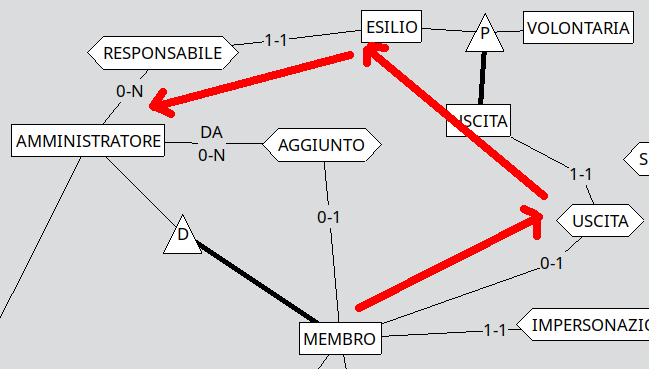
\includegraphics[scale=0.5]{./img/esilio.png}
\subsection{Ricostruire ricorsivamente le regioni superiori di una data regione} \label{aggiungere_regione}
\paragraph{Descrizione} Si percorre riscorsivamente il cammino che parte dalla regione data fino alla radice dell'albero attraversando tutte le regioni padre della regione data. 
\paragraph{Frequenza} 1 / 100 g
\paragraph{\texttt{NOTA}} Nel calcolo degli accessi abbiamo posto come ipotesi che l'altezza massima di questo albero sia 7. 
\begin{table}[H]
\paragraph{Tavola degli accessi\newline}
\begin{tabular}{|c|c|c|c|}
\hline
Concetto           & Costrutto  & Accessi    & Tipo       \\ \hline
REGIONE   & E & 7 & R \\ \hline
PARTE\_DI & A & 7 & R \\ \hline
TOTALE             &            & 14         &            \\ \hline
\end{tabular}
\end{table}
\section{Raffinamento dello schema}
\subsection{Eliminazione di gerarchie}
Nel nostro social network, un contenuto puo essere sia un 
post che un messaggio. Dato che i messaggi non hanno un titolo, mentre un post ha necessariamente un titolo, 
abbiamo optato definirli attraverso la presenza questo attributo, usando un collasso verso l' alto.
Un utente puo essere un amministratore o no in una chat, e anche in questo caso abbiamo optato per un collasso verso 
l' alto. Infatti, abbiamo inserito creato una table amminitratori, e se il membro presente in questa tabella allora quel membro è anche un amminsitratore. Questo ci permette di usare il vincolo referenziale per garantire che le operazioni che sono di esclusica competenza degli amministratori siano svolte solo da loro. 
\subsection{Numero di like netto dei contenuti}
Consideriamo se è il caso di aggiungere un campo ridondante nell'entità CONTENUTO che calcola il numero netto di like riguardanti quel contenuto. Le operazioni interessate da questa ridondanza sono le operazioni \ref{like}, \ref{leggere_post}, \ref{feed}.
\subsubsection{Caso senza ridondanza}
\begin{table}[H]
\paragraph{Operazione \ref{like}\newline}
\begin{tabular}{|c|c|c|c|}
\hline
Concetto        & Costrutto & Accessi & Tipo \\ \hline
UTENTE          & E         & 1       & R    \\ \hline
REAZIONE        & A         & 1       & W    \\ \hline
CONTENUTO       & E         & 1       & R    \\ \hline
\textit{TOTALE} &           & 4       &      \\ \hline
\end{tabular}
\end{table}
\begin{table}[H]
\paragraph{Operazione \ref{leggere_post}\newline}
\begin{tabular}{|c|c|c|c|}
\hline
Concetto             & Costrutto & Accessi & Tipo \\ \hline
CONTENUTO            & E         & 1       & R    \\ \hline
REAZIONE             & A         & 200     & R    \\ \hline
PUBBLICAZIONE        & A         & 1       & R    \\ \hline
UTENTE               & E         & 1       & R    \\ \hline
LUOGO\_PUBBLICAZIONE & A         & 1       & R    \\ \hline
REGIONE              & E         & 7       & R    \\ \hline
PARTE\_DI            & E         & 7       & R    \\ \hline
RISPOSTA             & A         & 10      & R    \\ \hline
COMMENTO             & E         & 10      & R    \\ \hline
REAZIONE             & A         & 2000    & R    \\ \hline
TOTALE               &           & 2238    &      \\ \hline
\end{tabular}
\end{table}
\begin{table}[H]
\paragraph{Operazione \ref{feed}\newline}
\begin{tabular}{|c|c|c|c|}
\hline
Concetto      & Costrutto & Accessi & Tipo \\ \hline
UTENTE        & E         & 1       & R    \\ \hline
SEGUE         & A         & 100     & R    \\ \hline
SEGUIRE       & E         & 100     & R    \\ \hline
SEGUITO       & A         & 100     & R    \\ \hline
UTENTE        & E         & 100     & R    \\ \hline
PUBBLICAZIONE & A         & 2000    & R    \\ \hline
CONTENUTO     & E         & 2000    & R    \\ \hline
REAZIONE      & A         & 400000  & R    \\ \hline
TOTALE        &           & 404401  &      \\ \hline
\end{tabular}
\end{table}
Il costo giornaliero di queste 3 operazioni in totale:
\begin{equation}
  \frac{80} g \times 4 R + \frac{100} g \times 2.238 R + \frac{40} g \times 404.401 R = 16.400.160 \frac{R} g 
\end{equation}
\subsubsection{Caso con ridondanza}
\begin{table}[H]
\paragraph{Operazione \ref{like}\newline}
\begin{tabular}{|c|c|c|c|}
\hline
Concetto        & Costrutto & Accessi & Tipo \\ \hline
UTENTE          & E         & 1       & R    \\ \hline
REAZIONE        & A         & 1       & W    \\ \hline
CONTENUTO       & E         & 2       & W    \\ \hline
\textit{TOTALE} &           & 5       &      \\ \hline
\end{tabular}
\end{table}
\begin{table}[H]
\paragraph{Operazione \ref{leggere_post}\newline}
\begin{tabular}{|c|c|c|c|}
\hline
Concetto             & Costrutto & Accessi & Tipo \\ \hline
CONTENUTO            & E         & 1       & R    \\ \hline
PUBBLICAZIONE        & A         & 1       & R    \\ \hline
UTENTE               & E         & 1       & R    \\ \hline
LUOGO\_PUBBLICAZIONE & A         & 1       & R    \\ \hline
REGIONE              & E         & 7       & R    \\ \hline
PARTE\_DI            & E         & 7       & R    \\ \hline
RISPOSTA             & A         & 10      & R    \\ \hline
COMMENTO             & E         & 10      & R    \\ \hline
TOTALE               &           & 38      &      \\ \hline
\end{tabular}
\end{table}
\begin{table}[H]
\paragraph{Operazione \ref{feed}\newline}
\begin{tabular}{|c|c|c|c|}
\hline
Concetto      & Costrutto & Accessi & Tipo \\ \hline
UTENTE        & E         & 1       & R    \\ \hline
SEGUE         & A         & 100     & R    \\ \hline
SEGUIRE       & E         & 100     & R    \\ \hline
SEGUITO       & A         & 100     & R    \\ \hline
UTENTE        & E         & 100     & R    \\ \hline
PUBBLICAZIONE & A         & 2000    & R    \\ \hline
CONTENUTO     & E         & 2000    & R    \\ \hline
TOTALE        &           & 4401    &      \\ \hline
\end{tabular}
\end{table}
Il costo giornaliero di queste 3 operazioni in totale:
\begin{equation}
  \frac{80} g \times 5 R + \frac{100} g \times 38 R + \frac{40} g \times 4.401 R = 180.440 \frac{R} g 
\end{equation}
Concludiamo che dobbiamo preservare la ridondanza.

\subsection{Numero di follower di un utente}
Consideriamo la possibilità di avere un campo ridondante nel profilo utente con il numero di utenti che seguono questo utente. Le operazioni interessate sono \ref{follow}, \ref{unfollow} e \ref{vedere_profilo}.
\subsubsection{Caso senza ridondanza}
\begin{table}[H]
  \paragraph{Operazione \ref{follow}\newline}
\begin{tabular}{|c|c|c|c|}
\hline
Concetto & Costrutto & Accessi & Tipo \\ \hline
UTENTE   & E         & 1       & R    \\ \hline
SEGUE    & A         & 1       & W    \\ \hline
SEGUIRE  & E         & 1       & W    \\ \hline
UTENTE   & E         & 1       & R    \\ \hline
TOTALE   &           & 6       &      \\ \hline
\end{tabular}
\end{table}
\begin{table}[H]
  \paragraph{Operazione \ref{unfollow}\newline}
\begin{tabular}{|c|c|c|c|}
\hline
Concetto & Costrutto & Accessi & Tipo \\ \hline
UTENTE   & E         & 1       & R    \\ \hline
SEGUE    & A         & 1       & R    \\ \hline
SEGUIRE  & E         & 1       & W    \\ \hline
UTENTE   & E         & 1       & R    \\ \hline
TOTALE   &           & 5       &      \\ \hline
\end{tabular}
\end{table}

\begin{table}[H]
\paragraph{Tavola degli accessi\newline}
\begin{tabular}{|c|c|c|c|}
\hline
Concetto & Costrutto & Accessi & Tipo \\ \hline
UTENTE   & E         & 1       & R    \\ \hline
SEGUE    & A         & 100     & R    \\ \hline
TOTALE   &           & 101     &      \\ \hline
\end{tabular}
\end{table}

Il costo giornaliero di queste 3 operazioni in totale:
\begin{equation}
  \frac{2} g \times 6 R + \frac{1} {10g} \times 5 R + \frac{5} g \times 101 R = 517,5 \frac{R} g 
\end{equation}

\subsubsection{Caso con ridondanza}
\begin{table}[H]
  \paragraph{Operazione \ref{follow}\newline}
\begin{tabular}{|c|c|c|c|}
\hline
Concetto & Costrutto & Accessi & Tipo \\ \hline
UTENTE   & E         & 1       & R    \\ \hline
SEGUE    & A         & 1       & W    \\ \hline
SEGUIRE  & E         & 1       & W    \\ \hline
UTENTE   & E         & 1       & W    \\ \hline
TOTALE   &           & 7       &      \\ \hline
\end{tabular}
\end{table}
\begin{table}[H]
  \paragraph{Operazione \ref{unfollow}\newline}
\begin{tabular}{|c|c|c|c|}
\hline
Concetto & Costrutto & Accessi & Tipo \\ \hline
UTENTE   & E         & 1       & R    \\ \hline
SEGUE    & A         & 1       & R    \\ \hline
SEGUIRE  & E         & 1       & W    \\ \hline
UTENTE   & E         & 1       & W    \\ \hline
TOTALE   &           & 6       &      \\ \hline
\end{tabular}
\end{table}
\begin{table}[H]
  \paragraph{Operazione \ref{vedere_profilo}\newline}
\begin{tabular}{|c|c|c|c|}
\hline
Concetto & Costrutto & Accessi & Tipo \\ \hline
UTENTE   & E         & 1       & R    \\ \hline
TOTALE   &           & 1       &      \\ \hline
\end{tabular}
\end{table}
Il costo giornaliero di queste 3 operazioni in totale:
\begin{equation}
  \frac{2} g \times 7 R + \frac{1} {10g} \times 6 R + \frac{5} g \times 1 R = 19,6 \frac{R} g 
\end{equation}
Alla luce di ciò abbiamo scelto di preservare la ridondanza.
\subsection{Reputazione di un utente}
Consideriamo la possibilità di aggiunge un campo ridondante che tenga conto della reputazione attuale di un utente. Ricordiamo che la reputazione di un utente è la somma algebrica dei like dati ai contenuti pubblicati da quel utente.
Le operazioni interessate dalla ridondanza sono \ref{like} e \ref{vedere_profilo}.
\subsubsection{Caso senza ridondanza}
\begin{table}[h]
  \paragraph{Operazione \ref{like}\newline}
\begin{tabular}{|c|c|c|c|}
\hline
Concetto        & Costrutto & Accessi & Tipo \\ \hline
UTENTE          & E         & 1       & R    \\ \hline
REAZIONE        & A         & 1       & W    \\ \hline
CONTENUTO       & E         & 1       & W    \\ \hline
\textit{TOTALE} &           & 5       &      \\ \hline
\end{tabular}
\end{table}

\begin{table}[H]
  \paragraph{Operazione \ref{vedere_profilo}\newline}
\begin{tabular}{|c|c|c|c|}
\hline
Concetto & Costrutto & Accessi & Tipo \\ \hline
UTENTE   & E         & 1       & R    \\ \hline
REAZIONE & A         & 2000    & R    \\ \hline
TOTALE   &           & 2001    &      \\ \hline
\end{tabular}
\end{table}
Quindi il costo totale giornaliero è:
\begin{equation}
  \frac{80} g \times 5 R + \frac{5} {g} \times 2001 R = 10405 \frac{R} g 
\end{equation}

\subsubsection{Caso con ridondanza}
\begin{table}[h]
  \paragraph{Operazione \ref{like}\newline}
\begin{tabular}{|c|c|c|c|}
\hline
Concetto        & Costrutto & Accessi & Tipo \\ \hline
UTENTE          & E         & 1       & R    \\ \hline
REAZIONE        & A         & 1       & W    \\ \hline
CONTENUTO       & E         & 1       & W    \\ \hline
PUBBLICAZIONE   & A         & 1       & W    \\ \hline 
UTENTE          & E         & 1       & W    \\ \hline
\textit{TOTALE} &           & 9       &      \\ \hline
\end{tabular}
\end{table}

\begin{table}[H]
  \paragraph{Operazione \ref{vedere_profilo}\newline}
\begin{tabular}{|c|c|c|c|}
\hline
Concetto & Costrutto & Accessi & Tipo \\ \hline
UTENTE   & E         & 1       & R    \\ \hline
TOTALE   &           & 1       &      \\ \hline
\end{tabular}
\end{table}
Quindi il costo totale giornaliero è:
\begin{equation}
  \frac{80} g \times 9 R + \frac{5} {g} \times 1 R = 725 \frac{R} g 
\end{equation}
In luce di ciò abbiamo deciso di mantenere la ridondanza.

\section{Traduzione di entità e associazioni in relazioni}
Abbiamo ovviamente trasformato tutte le entità del modello concettuale in relazione, mentre per quanto riguadarda le associazioni nessuna di loro è stata trasformata tranne REAZIONE, cioè l'unica che aveva come cardinalità (0,N), (0, N), Tuttel le altre sono del tipo uno a molti, perciò abbiamo deciso di tradurle in attributi delle entità dal lato dell'uno. L'assenza di molte associazioni molti a molti non ci stupisce perchè molte di queste relazioni sono state reificate per supportare il sviluppo temporale di queste associazioni. Un esempio di queste è l'entità SEGUIRE, la quale era in prima analisi una associazione, ma successivamente ci siamo posti il problema di avere tutta la storia di come gli utenti inizino a seguirsi, smettono e ricominciano.
\section{Schema relazionale finale}
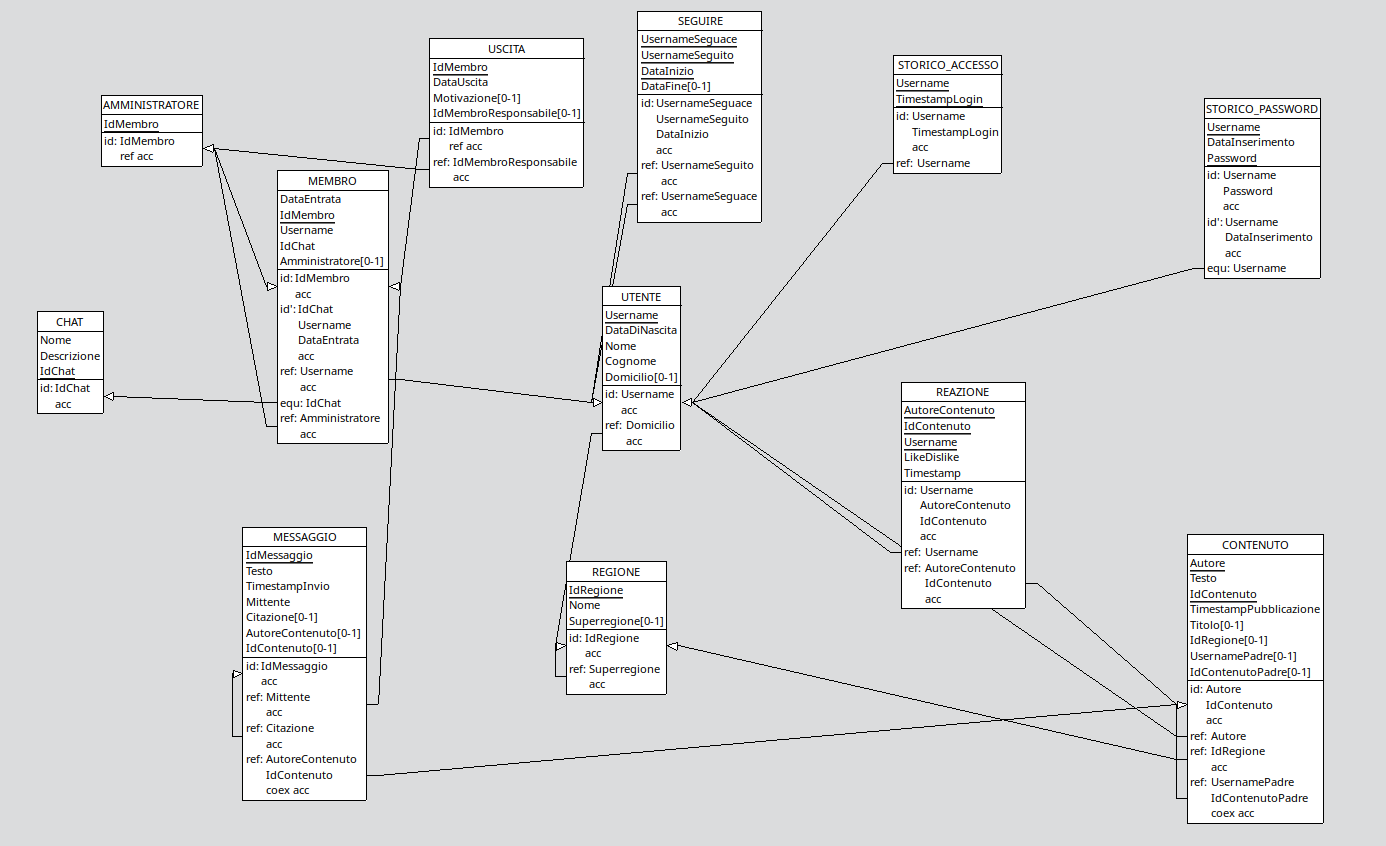
\includegraphics[scale=0.6, angle=90]{./img/logico.png}
\section{Traduzione delle operazioni in query SQL}
\subsection{Creazione  tabelle}
\begin{lstlisting}
  -- Database Section
  -- ________________ 
  
  
  
  -- Tables Section
  -- _____________ 
  
  create table AMMINISTRATORE (
       IdMembro integer not null,
       constraint FKAMMINISTRATORE_ID primary
        key (IdMembro));
  
  create table CHAT (
       Nome varchar(100) not null,
       Descrizione varchar(5000) not null,
       IdChat serial not null,
       constraint ID_CHAT_ID primary key (IdChat));
  
  create table CONTENUTO (
       Autore varchar(20) not null,
       Testo varchar(1000) not null,
       IdContenuto serial not null,
       TimestampPubblicazione date not null,
       Titolo varchar(30),
       IdRegione integer, 
       UsernamePadre varchar(20),
       IdContenutoPadre integer,
       LikeDelta integer not null,
       constraint ID_CONTENUTO primary key
        (Autore, IdContenuto));
  
  create table MEMBRO (
       DataEntrata date not null,
       IdMembro serial not null,
       Username varchar(20) not null,
       IdChat integer not null,
       Amministratore integer,
       constraint ID_MEMBRO primary key (IdMembro),
       constraint SID_MEMBRO unique 
       (IdChat, Username, DataEntrata));
  
  create table MESSAGGIO (
       IdMessaggio serial not null,
       Testo varchar(1000) not null,
       TimestampInvio date not null,
       Mittente integer not null,
       Citazione integer,
       AutoreContenuto varchar(20),
       IdContenuto integer,
       AmministratoreEliminatore integer,
       constraint ID_MESSAGGIO primary key
        (IdMessaggio));
  
  create table REAZIONE (
       AutoreContenuto varchar(20) not null,
       IdContenuto integer not null,
       Username varchar(20) not null,
       LikeDislike integer not null,
       Timestamp timestamp not null,
       constraint ID_REAZIONE primary key
        (Username, AutoreContenuto, IdContenuto));
  
  create table REGIONE (
       IdRegione serial not null,
       Nome varchar(50) not null,
       Superregione integer,
       constraint ID_REGIONE primary key (IdRegione));
  
  ALTER sequence REGIONE_IdRegione_seq 
    MINVALUE 0 RESTART WITH 0;
  
  create table SEGUIRE (
       UsernameSeguace varchar(20) not null,
       UsernameSeguito varchar(20) not null,
       DataInizio date not null,
       DataFine date,
       constraint ID_SEGUIRE primary key 
        (UsernameSeguace, UsernameSeguito, DataInizio),
       constraint DataInizioMinDataFine CHECK 
       (DataInizio < DataFine),
       constraint SeguireNonSeStessi CHECK 
        (UsernameSeguace <> UsernameSeguito));
        
  create table STORICO_ACCESSO (
       Username varchar(20) not null,
       TimestampLogin timestamp not null,
       constraint ID_STORICO_ACCESSO 
        primary key (Username, TimestampLogin));
  
  create table STORICO_PASSWORD (
       Username varchar(20) not null,
       DataInserimento timestamp not null,
       Password varchar(20) not null,
       constraint SID_STORICO_PASSWORD unique 
        (Username, DataInserimento),
       constraint ID_STORICO_PASSWORD 
        primary key (Username, Password));
  
  create table USCITA (
       IdMembro integer not null,
       DataUscita date not null,
       Motivazione varchar(500),
       IdMembroResponsabile integer,
       constraint FKUSCITA_ID primary key (IdMembro));
  
  create table UTENTE (
       Username varchar(20) not null,
       DataDiNascita date,
       Nome varchar(20),
       Cognome varchar(20),
       Domicilio integer,
       NumeroSeguaci integer not null,
       constraint ID_UTENTE_ID primary key (Username));
  
  
  -- Constraints Section
  -- ___________________ 
  
  alter table AMMINISTRATORE add constraint 
  FKAMMINISTRATORE_FK
       foreign key (IdMembro)
       references MEMBRO;
  
  alter table CONTENUTO add constraint FKPUBBLICAZIONE
       foreign key (Autore)
       references UTENTE;
  
  alter table CONTENUTO add constraint
   FKLUOGO_PUBBLICAZIONE_FK
       foreign key (IdRegione)
       references REGIONE;
  
  alter table CONTENUTO add constraint FKRISPOSTA_FK
       foreign key (UsernamePadre, IdContenutoPadre)
       references CONTENUTO;
  
  alter table CONTENUTO add constraint FKRISPOSTA_CHK
       check((UsernamePadre is not null and 
              IdContenutoPadre is not null)
             or (UsernamePadre is null and
                IdContenutoPadre is null)); 
  
  alter table MEMBRO add constraint FKIMPERSONAZIONE_FK
       foreign key (Username)
       references UTENTE;
  
  alter table MEMBRO add constraint FKAPPARTENENZA
       foreign key (IdChat)
       references CHAT;
  
  alter table MEMBRO add constraint FKAGGIUNTO_FK
       foreign key (Amministratore)
       references AMMINISTRATORE;
  
  alter table MESSAGGIO add constraint FKMITTENTE_FK
       foreign key (Mittente)
       references MEMBRO;
  
  alter table MESSAGGIO add constraint FKCITAZIONE_FK
       foreign key (Citazione)
       references MESSAGGIO;
  
  alter table MESSAGGIO add constraint FKRIFERIMENTO_FK
       foreign key (AutoreContenuto, IdContenuto)
       references CONTENUTO;
  
  alter table MESSAGGIO add constraint 
  FKRIFERIMENTO_CHK
       check((AutoreContenuto is not null and
        IdContenuto is not null)
             or (AutoreContenuto is null
              and IdContenuto is null)); 
  
  alter table MESSAGGIO 
  add constraint FKELIMINAZIONE_FK
       foreign key (AmministratoreEliminatore)
       references AMMINISTRATORE;
  
  alter table REAZIONE add constraint FKREA_UTE
       foreign key (Username)
       references UTENTE;
  
  alter table REAZIONE add constraint FKREA_CON_FK
       foreign key (AutoreContenuto, IdContenuto)
       references CONTENUTO;
  
  alter table REGIONE add constraint FKPARTE_DI_FK
       foreign key (Superregione)
       references REGIONE;
  
  alter table SEGUIRE add constraint FKSEGUITO_FK
       foreign key (UsernameSeguito)
       references UTENTE;
  
  alter table SEGUIRE add constraint FKSEGUE_FK
       foreign key (UsernameSeguace)
       references UTENTE;
  
  alter table STORICO_ACCESSO add constraint FKACCESSO
       foreign key (Username)
       references UTENTE;
  
  alter table STORICO_PASSWORD add constraint FKSCELTA
       foreign key (Username)
       references UTENTE;
  
  alter table USCITA add constraint FKUSCITA_FK
       foreign key (IdMembro)
       references MEMBRO;
  
  alter table USCITA add constraint FKRESPONSABILE_FK
       foreign key (IdMembroResponsabile)
       references AMMINISTRATORE;
  
  alter table UTENTE add constraint FKDOMICILIO_FK
       foreign key (Domicilio)
       references REGIONE;
  
  
\end{lstlisting}
\subsection{Operazioni utente}
Creare nuovo utente
\begin{lstlisting}
  -- name: InsertUser :exec
INSERT INTO UTENTE (Username, 
DataDiNascita, Nome, Cognome, Domicilio, NumeroSeguaci) 
  VALUES ($1,$2,$3, $4, $5, 0);

\end{lstlisting}

Cambiare password utente
\begin{lstlisting}
-- name: InsertPassword :exec
INSERT INTO STORICO_PASSWORD (Username, Password,
 DataInserimento) VALUES ($1, $2, $3);
\end{lstlisting}

Seguire utente
\begin{lstlisting}
-- name: InsertFollower :exec
INSERT INTO SEGUIRE 
(UsernameSeguace, UsernameSeguito, DataInizio, DataFine)
  VALUES ($1, $2, $3, $4);
\end{lstlisting}

Mandare un messaggio
\begin{lstlisting}
-- name: InsertMessage :exec
INSERT INTO MESSAGGIO 
(Testo, TimestampInvio, Mittente) VALUES ($1, $2, $3);
\end{lstlisting}

Postare e commentare
\begin{lstlisting}
  -- name: InsertComment :exec
INSERT INTO CONTENUTO (
  Autore, Testo, TimestampPubblicazione, 
  IdRegione, UsernamePadre, IdContenutoPadre, LikeDelta
) VALUES ($1, $2, $3, $4, $5, $6, 0);
\end{lstlisting}

Like 
\begin{lstlisting}
  - name: PutLike :exec
INSERT INTO REAZIONE ( 
  autorecontenuto, IdContenuto, username,
   likedislike, timestamp)
VALUES ($1, $2, $3, $4, $5)
ON CONFLICT (autorecontenuto, IdContenuto,
 username) DO UPDATE SET 
      likedislike = excluded.likedislike,
      timestamp = excluded.timestamp;'
\end{lstlisting}

Aggiungere utente al gruppo  (non operazione utente?)
\begin{lstlisting}
  -- name: InsertMember :one
  INSERT INTO MEMBRO (
    DataEntrata, Username, IdChat, Amministratore
  ) VALUES ( $1, $2, $3, $4 )
  RETURNING IdMembro;
\end{lstlisting}
Vedere tutti i post in ordine cronologico (feed)

\begin{lstlisting}
-- name: GetFullFeed :many
SELECT titolo, autore, IdContenuto, 
TimestampPubblicazione, Testo FROM SEGUIRE 
JOIN CONTENUTO ON 
CONTENUTO.Autore = SEGUIRE.usernameSeguito  
WHERE SEGUIRE.usernameseguace = ($1) AND
 datafine IS NULL AND IdContenutoPadre IS NULL;
\end{lstlisting}

Leggere messaggi di una chat
\begin{lstlisting}
-- name: GetChatMessages :many
SELECT testo, TimestampInvio, username 
FROM MESSAGGIO JOIN MEMBRO ON 
MEMBRO.IdMembro = MESSAGGIO.Mittente
 WHERE MEMBRO.idChat = $1;
 
\end{lstlisting}

Login utente
\begin{lstlisting}
  -- name: Authenticate :one
  SELECT COUNT(SUBQUERY.DataInserimento)
  FROM (
     SELECT MIN(SP.DataInserimento) AS DataInserimento
     FROM STORICO_PASSWORD SP 
     WHERE SP.Username = $1 AND SP.Password = $2
  ) AS SUBQUERY;
\end{lstlisting}

Vedere profilo utente
Dare diritti amministratore ad utente
\begin{lstlisting}
  -- name: InsertAdmin :exec
INSERT INTO AMMINISTRATORE (
  IdMembro
) VALUES ( $1 );
\end{lstlisting}

\chapter{Progettazione dell'applicazione}
\section{Descrizione dell'architettura dell'applicazione e alcuni screenshot dell'interfaccia utente}
Abbiamo progettato l'applicazione cercando di tenere divisi le responsabilità di view da quelle del model. 
Perciò abbiamo sviluppato una struct \texttt{Model} che ha dei metodi che permettono di eseguire tutte le operazioni sul database. 
La view invece usa le funzionalità del model e grazie alla funzionalità di Go di implementare implicitamente le interfacce permetettiamo ai vari componenti della view di dichiarare delle loro piccole interfacce private che esplicassero solo le funzionalità del model di cui hanno bisogno, usando il concetto di interfacce implicite di go.
Abbiamo introdotto dei check di base nella view (ad esempio non e possibile inserire password vuote nella view di registrazione), ma abbiamo preferito il piu possibile
di inserire direttamente questi constraint a livello di schema.
\newline

Registrazione:
\newline
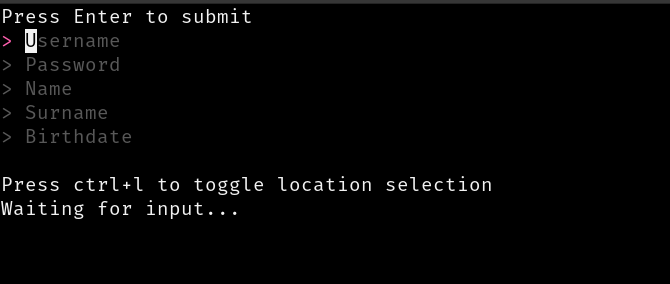
\includegraphics[width=10cm]{img/signup.png}
\newline
Visualizzazione di un post:
\newline
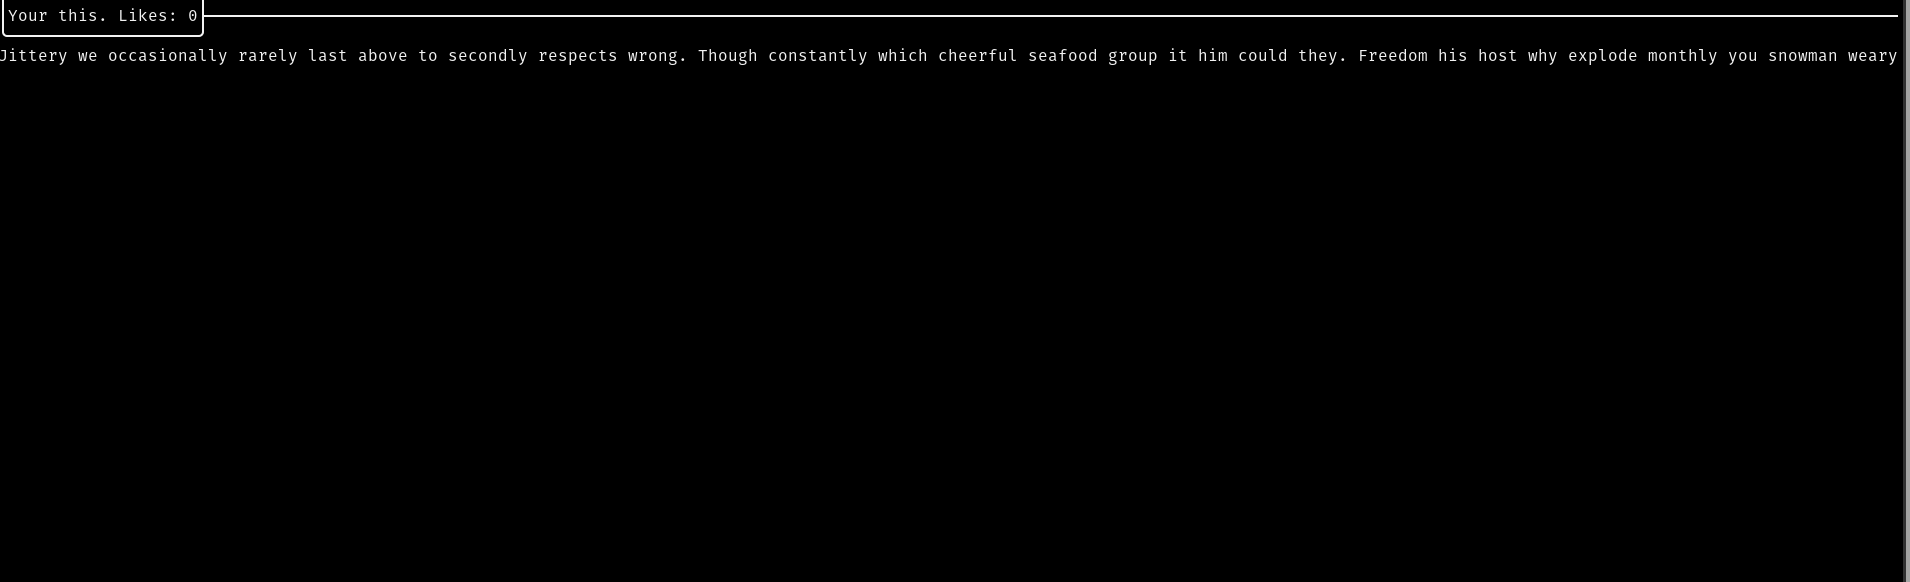
\includegraphics[height=6cm]{img/post_view.png}
\newline
Selezione chat:
\newline
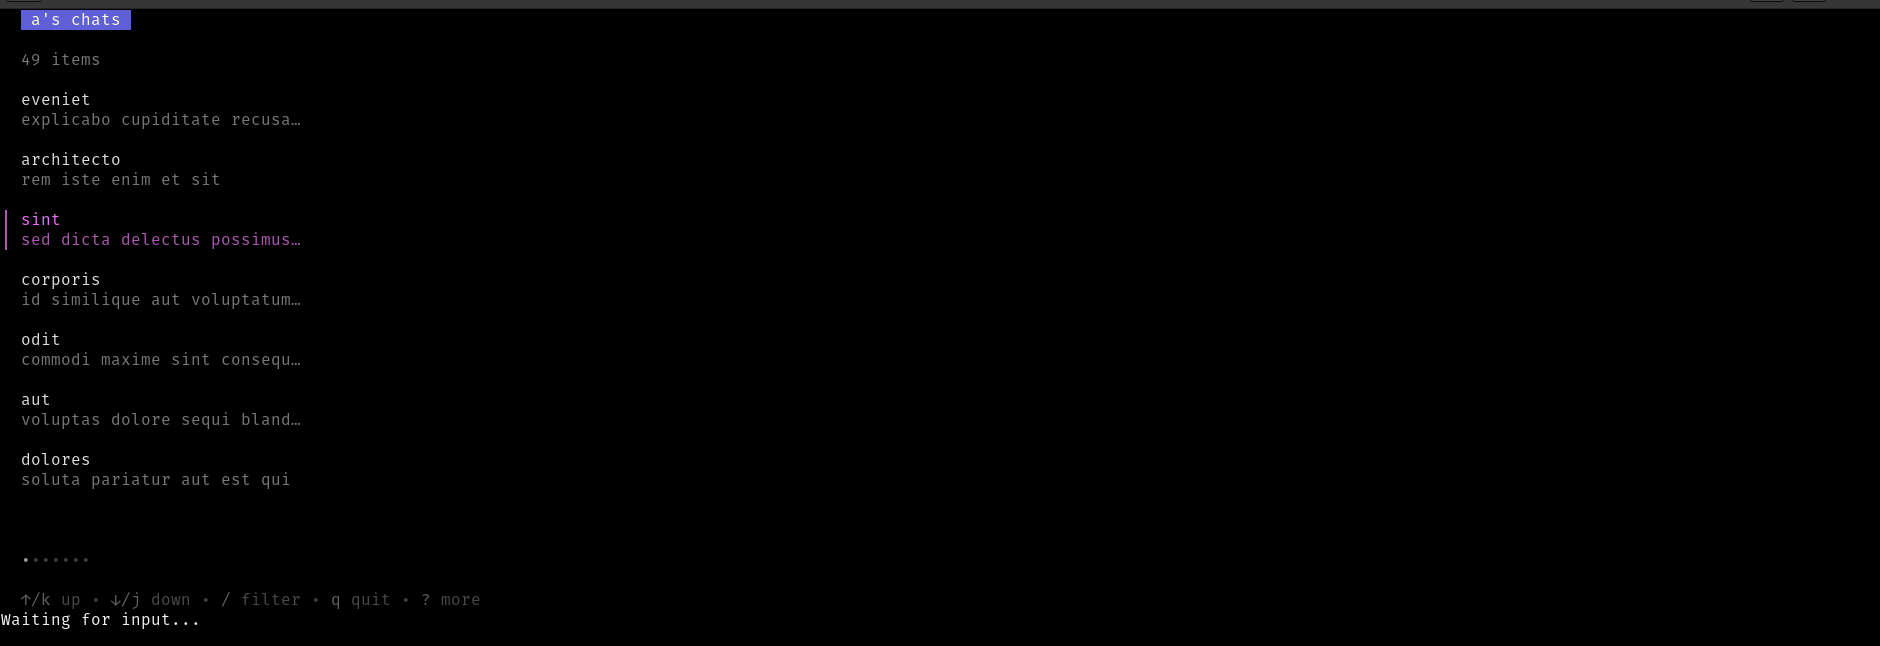
\includegraphics[height=5cm]{img/chats_view.png}
Chat singola:
\newline
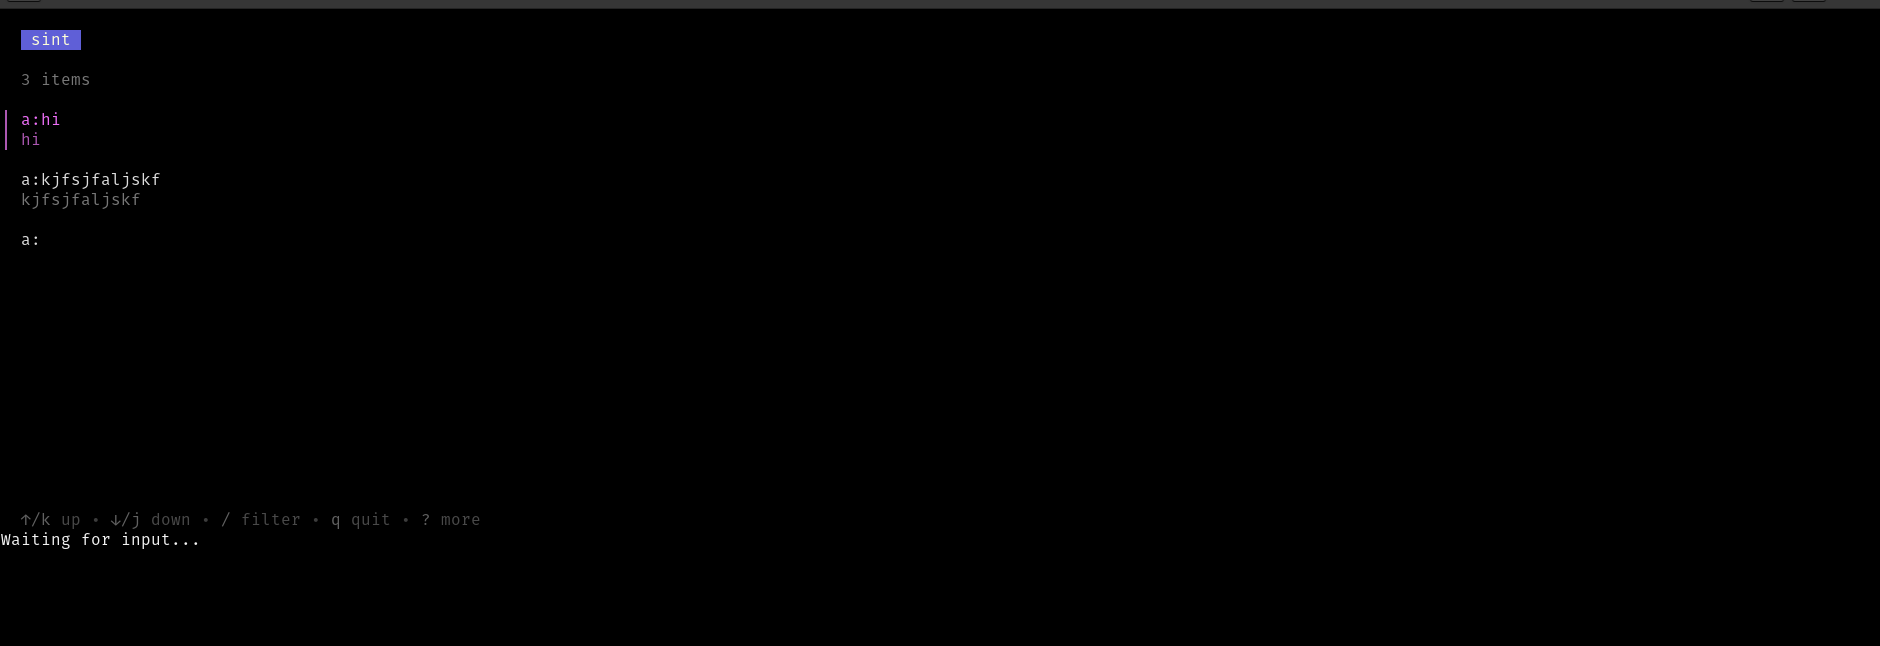
\includegraphics[height=5cm]{img/single_chat_view.png}
\newline
\end{document}
